\documentclass[conference]{IEEEtran}
% Add the compsoc option for Computer Society conferences.
%
% If IEEEtran.cls has not been installed into the LaTeX system files,
% manually specify the path to it like:
% \documentclass[conference]{../sty/IEEEtran}

% Some very useful LaTeX packages include:
% (uncomment the ones you want to load)

%
\usepackage{graphicx}





% correct bad hyphenation here
\hyphenation{op-tical net-works semi-conduc-tor}


\begin{document}
%

\title{Behavioral Correlation: A new approach for clustering sensors in Wireless Sensor Networks}

% author names and affiliations
% use a multiple column layout for up to three different
% affiliations
\author{\IEEEauthorblockN{Fernando Rodrigues}
\IEEEauthorblockA{University of Fortaleza\\Fortaleza - Ceara - Brazil\\
fernandorodrigues@edu.unifor.br}
\and
\IEEEauthorblockN{Angelo Brayner}
\IEEEauthorblockA{University of Fortaleza\\
Fortaleza - Ceara - Brazil\\
brayner@unifor.br}
\and
\IEEEauthorblockN{Jose E. Bessa Maia}
\IEEEauthorblockA{State University of Ceara\\
Fortaleza - Ceara - Brazil\\
jose.maia@uece.br}}


% make the title area
\maketitle


\begin{abstract}

Sensor clustering is an efficient strategy to reduce the number of messages
transmitted to the sink in a multi-hop Wireless Sensor Network.
In this work, we present a new approach to cluster sensors in WSN, denoted
Behavioral Correlation in WSN (BCWSN), based on the behave of recent historical
data collected by sensors. Instead of using the spatial distance among sensors
for clustering them, the proposed approach uses the concept of behavioral
correlation to group sensors, that takes into account the concepts of difference
in magnitude and trend of sensed data.
Furthermore, two scheduling intra-clustering methods are presented:
Representative Nodes and Cluster Heads.
In order to validate our approach, simulations with a prototype have been
conducted over real temperature data. The results show that, with 5\% error
threshold in temporal prediction, BCWSN can save the communication overhead up
to 97.72\% over naive strategy and 69.02\% over a temporal correlation approach,
while the RMSE remains roughly stable.

% The results point to gains of up to 97.72\% over naive strategy in terms of
% reduction in message transmission and 45,12\% of reduction in data sensing,
% while the RMSE remains roughly stable. To the best of our knowledge, we believe
% that our proposal brings gains in energy efficiency for WSNs.

% The best way to improve prediction accuracy is by decreasing prediction errors,
% using the same energy amount than the second version, but there is a trade-off
% between prediction accuracy and energy consumption.

\end{abstract}

% IEEEtran.cls defaults to using nonbold math in the Abstract.
% This preserves the distinction between vectors and scalars. However,
% if the conference you are submitting to favors bold math in the abstract,
% then you can use LaTeX's standard command \boldmath at the very start
% of the abstract to achieve this. Many IEEE journals/conferences frown on
% math in the abstract anyway.

% no keywords




% For peer review papers, you can put extra information on the cover
% page as needed:
% \ifCLASSOPTIONpeerreview
% \begin{center} \bfseries EDICS Category: 3-BBND \end{center}
% \fi
%
% For peerreview papers, this IEEEtran command inserts a page break and
% creates the second title. It will be ignored for other modes.
\IEEEpeerreviewmaketitle



\section{Introduction}
% no \IEEEPARstart


Sensors are devices used to collect data from the environment related to the
detection or measurement of physical phenomena. Sensors are limited in power,
computational capacity, and memory. Advances in wireless communication have
enabled the development of massive-scale wireless sensor networks (WSN). In a
WSN, sensors are usually scattered in the network and use low-power
communication channels. Thus, sensors disseminate collected data to a base
station, from where the information (query) was originally requested. Wireless
sensor networks (WSNs) have been widely used for environmental monitoring (e.g.,
traffic, habitat), industrial sensing and diagnostics (e.g., factory, supply
chains), infrastructure protection (e.g., water distribution), battlefield
awareness (e.g., multi-target tracking) and context-aware computing (e.g.,
intelligent home) applications.

In spite of advances in WSN technology, a critical key point is still the
energy consumption of sensor nodes. It is well known that communication among
sensors is the activity responsible for the bulk of the power consumption. By
reducing communication costs, energy may be drastically saved, consequently
increasing the WSN's lifetime. An effective strategy to reduce energy
consumption is thus to reduce the number of messages (sensed data) sent across
the network. Nevertheless, the less the number of sensed data is transmitted,
the lower the accuracy of results provided by a WSN is. Thus higher accuracy in
WSNs comes at a higher energy cost.

By now, it is well-known that data collected by WSN are strongly temporally
and/or spatial correlated \cite{Yoon2005, Chu2006}. The traditional spatial data
correlation is related to the idea that the physical proximity among sensors
leads to similar measurements (values) of sensed data, phenomenon known as
"principle of spatial locality". Thus, one can infer that from the capture of
some sensors readings (located in some regions of sensing space), it is possible
to obtain, approximately, the values of the readings of other sensors in its
surroundings. On the other hand, the temporal correlation indicates the various
readings of a sensor within a time interval have a certain approximation of
their values (principle of temporal locality). such a feature makes possible to
predict (with a certain margin of error) sensed values in the future based on
data collected in the past.

Grouping sensors in clusters is the main technique used to take advantage of the
principle of spatial locality for reducing the energy consumption in WSNs. This
is because one can use only a few representative nodes from each cluster to
sense data in a given spatial region (cluster) in which sensors are spatially
correlated.
Several works have been proposed in order to use that technique, with different
approaches \cite{Chu2006, Villas2012, Singh2010, Liu2007, Shah2007}.

Nonetheless, in several scenarios sensors, which are not spatially close to each
other, may have similar data reading patterns. In order to illustrate such a
claim consider a dense WSN deployed to monitor forest fires. 
Now, suppose a scenario in which the monitored region is affected by dozens of
small forest fires. Figure \ref{fig:contour_lines} depicts a possible temperature
contour lines graph for this hypothetical situation. Observe that the contour
lines in Figure \ref{fig:contour_lines} form several closed regions representing
areas which may have small forest fire areas, where it is very likely that the
temperature measurements of sensors in those spatially separated regions present
high correlation. For that reason, we claim that in such cases, a better
alternative would be to use sensor clustering strategy based on
\textit{Behavioral Correlation}.

The idea behind the concept of {\it Behavioral Correlation} is to identify
similar patterns of sensor readings even in sensors which are geographically
distant from each other. Thus, one could apply a Behavioral Correlation
Clustering (BCC) technique to group sensors which are spatially separated into a
single cluster, in contrast to existing spatio-temporal correlation techniques.
The BCC technique clusters sensors for which the forecasting models of sensed
data time series are approximately the same independent of spatial proximity of
sensors.

\begin{figure}[!htb]
\centering
	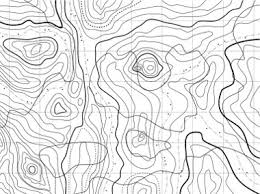
\includegraphics[scale=0.9]{I2.png}
    \caption{Contours lines of temperature}
    \label{fig:contour_lines}
\end{figure}

In this sense, in this paper, we present a new approach for clustering sensors in
WSNs. The main features of the proposed approach are: {\it (i)} Cluster
formation based on the \textit{Behavioral Correlation} of the sensors, which, in
turn, is computed from the time series of sensor readings by applying a
\textit{Similarity Measure}, and; {\it (ii)} the use of a linear regression
model for the temporal suppression of sensed data through the maximum error
level (threshold) desired by the user used to control the data to be sent to the
sink. Hence, special sensor nodes only transmit data which are novelties for the
regression model applied by our proposal. Furthermore, two different approaches
to select of active nodes (scheduling) in each cluster have been implemented:
Representative Nodes (RNs) and Cluster Heads (CHs).


The remainder of this document is organized as follows. Section
\ref{related-work} describes related work and point out the differences between
our method and existing methods. In Section \ref{implementing-bcwsn} the
proposed Behavioral Correlation in WSN (BCWSN) method and two sensor-scheduling
policies are presented and discussed. Simulations with a Sinalgo prototype
operating over real sensor data are reported in Section \ref{eval}. Finally,
Section \ref{conclusion} concludes the paper.


\section{Related Work}
\label{related-work}

In \cite{Vuran2004}, proposes a strategy to cluster sensors in WSNs. The idea is
the following: given a set of N sensors, M nodes, with $M < N$, are chosen to
send data. The M representative nodes are defined based on the application of a
distortion function ($D(M)$) on sensed data.
The spatial distance between the nodes (representative) directly influences the
computation of the distortion function by means of a correlation coefficient.
That work does not take into account the energy capacity of each node as a
criterion for choosing representative nodes, although this is a very important
factor due to the restrictive characteristics regarding the energy consumption
of the nodes in a WSN.

In EAST \cite{Villas2012}, sensors are grouped into two levels, under a spatial
correlation approach, while the leader and the representative nodes perform a
temporal suppression technique.
The leader node generates a representative value for each cluster based on data
received by the representative nodes, which form a subset of all the nodes that
sense the same event. The sensed area is divided into "event areas", which in
turn are divided into "correlation regions (c) or cells", where the formers will
be managed, each one, for a "Coordinator node" and the "correlation areas" will
be represented, one by one, by a "Representative node" because a single reading
within this region is enough to represent it.
The size of the correlation region (c) can be decremented or incremented by the
sink according to the application and the characteristics of the event, to
maintain the accuracy of the data collected.

Another way to group sensor nodes into clusters is through measures of
dissimilarity.
In EEDC \cite{Liu2007}, such measures of dissimilarity are calculated by the
sink node for all pairs of nodes of the network, regardless of their location.
The measure of dissimilarity between two nodes is calculated based on up to $3$
parameters, namely:
the differences in magnitude (\textit{M}) and trend (\textit{T}) of the data
values and the geographical/euclidean distance between nodes ($g_{max}dist$).
The criterion of formation of clusters is based on the maximum threshold of
dissimilarity (max\_dst) defined by a tuple (\textit{M}, \textit{T},
$g_{max}dist$), based on the measure of dissimilarity between the nodes. It
works as follows: $1)$ Initially, the data sensed by each node are sent in the
form of a temporal series for the sink. $2)$ The sink then stores all the data
from the sensors and then calculates the measure of dissimilarity (previously
mentioned) for each pair of nodes of the network. $3)$ With the measures
calculated and the maximum threshold of dissimilarity (max\_dst), the sink
divides the nodes into clusters. 
That work does not takes into account the energy reserve of each node as a
criterion for choosing representative nodes (it is used an algorithm that makes,
simultaneously, the equitable scheduling - round robin - along with the random
choice of representatives nodes).

The spatial correlation through the formation of clusters is addressed in
\cite{Pham2010} in the form a flooding algorithm where the sink node starts to
send messages to the other nodes of the network, inviting them to form groups
from criteria such as a dissimilarity measure, in addition to the physical
proximity between nodes, since, of course, the message forwarding in a WSN
occurs between adjacent nodes (i.e. geographically close). Cluster Heads (CHs)
are selected, basically, by 2 parameters: {\it (i)} the nodes that are one hop
from the ancestor that sent the message calculate the measure of dissimilarity
with the mean value informed in the message and then those that are within the
threshold of dissimilarity if they apply for CH, where {\it (ii)} it is said to
be the CH the one that have higher level of energy reserve.
We should notice that, during the process of forming clusters, the nodes that
will form the communication backbone between each Cluster Head node and the sink
are also configured. A scheduling of each cluster is done through round robin in
order to decide which member node that will be active in each time slot making
the sensing and sending the data to its respective CH.
The weak point is the process of forming clusters, in
which there is an intensive exchange of messages, scattering a significant
amount of energy from the network sensors.

In \cite{Shah2007}, the spatial correlation is explored by a mechanism called
the GSC (Gridiron Spatial Correlation), where the sensed region has a Cluster
Head that will be in the center of the region delimited by r (radius of the
monitored region), which will be divided into correlated regular regions
(quadratic), according to the spatial density level chosen, defined through
$\theta$ (size of the correlation region equal to $\theta^2$). In this way,
active sensors will be chosen according to 2 basic parameters: {\it (i)} the
proximity of the them regarding the center of the regions correlated and {\it
(ii)} their energy level must be within a certain threshold, above the ones of
their closest neighbours. The scheduling of active nodes works through the
passage of a list by the cluster-head for all nodes with the nodes being active
in each time slot, where this configuration is only changed when one of the
active nodes has its energy level below the threshold established.
That work does not describe how the energy threshold is calculated neither how
this reconfiguration of the sizes of the rectangles are done and not even gives
examples of the that.


\section{Implementing Behavioral Correlation in WSNs}
\label{implementing-bcwsn}

In this section, we present the proposed approach for clustering sensors in a
WSN based on the notion of {\it Behavioral Correlation}. Our approach, called
Behavioral Correlation in Wireless Sensor Networks (\textit{BCWSN} for short),
is based on clustering sensors by means of behavioral correlation (descrived in
\ref{clustering-sensors}), which is in turn computed from the time series of
sensor readings, and on using a linear regression model for the temporal
suppression of data to be sent to the sink node.

Two different approaches for intra-cluster sensor node scheduling have been
implemented in order to uniformly distribute the sensing activity for the
sensor nodes of a cluster. In the first one, called Representative Nodes (RNs),
only one node in each cluster $C_{i}$ is chosen at each time to represent that
cluster. In other words, a representative node is responsible for sensing and
predicting data in $C_{i}$ for given time interval. In this case, we have a
greater energy economy in the network as a trade-off from a little
general precision, because changes in fenomena sensed at network positions where
the sensors are in stand-by mode (non-Representative Nodes) would not be
captured. To stand up to this weakness, we have a second method, called
Cluster Heads (CHs). In this other approach, on the other hand, one sensor node
(the CH) in each cluster $C_{i}$ is selected to coordinate the data sensing
activity carried out by all nodes in $C_{i}$. So, changes are promptly sensed by
active nodes, having major impact on energy expediture from nodes activation.

\subsection{The BCWSN Mechanism}


The algorithm BCWSN can be divided into five steps described next.


\subsubsection{Learning Stage}

In this step, the sink node collects sensed data from all sensors belonging to
the network in order to compute the initial cluster formation and the
coefficients of the linear regression equation (see Section \ref
{data-predict}). Thus, the sink node firstly sends a broadcast message to all
nodes of the network, requesting the following data from sensors:
battery level, spatial location and sensed values. The amount of data used by the
learning stage is a parameter, denoted initial slot time, which should be
defined by the application expert.


\subsubsection{Clustering Sensor Nodes}
\label{clustering-sensors}

As already mentioned, the CCWSN mechanism clusters sensor nodes by means of
behavioral correlation. In order to compute behavioral correlation, a
\textit{similarity measure} \cite{Liu2007} is used. Thus, sensors with similar
data reading pattern are grouped into a single cluster. The similarity measure
among sensed data of two different sensors is defined by  similarity of
magnitude and similarity of trend, defined next.

\newtheorem{defini}{Definition}

\begin{defini}
Similarity of magnitude-M: Two sensors ($S$ and $S'$) with time series
$S$=\{$s_{1}$,$s_{2}$,\ldots,$s_{n}$\} and
$S'$=\{$s'_{1}$,$s'_{2}$,\ldots,$s'_{n}$\} are magnitude-M similar if 
\begin{equation}
\label{equ:magni}
\frac{\sum_{i=1}^{n} |s_{i}-s'_{i}|}{n} \leq M
\end{equation}
%$\displaystyle \sum_{i = 0}^{n} |s_{1_i}-s_{2_i}| \leq M$
\end{defini}

\begin{defini}
Similarity of trend-T: Two sensors ($S$ and $S'$) with time series
$S$=\{$s_{1}$,$s_{2}$,\ldots,$s_{n}$\} and
$S'$=\{$s'_{1}$,$s'_{2}$,\ldots,$s'_{n}$\} are trend-T similar if 
\begin{equation}
\label{equ:trend}
\frac{P}{n} \geq T,
\end{equation}
where $n$ is the total number of sensed data and $P$ is the number of pairs
$(s_{i},s'_{i})$ in the time series which satisfy $\nabla s_{i} \times \nabla
s'_{i} \geq 0$, where $\nabla s_{i} = s_{i} - s_{i-1}$, $\nabla
s'_{i} = s'_{i} - s'_{i-1}$ and $1 < i \leq n$.
\end{defini}

Thus, sensors which are magnitude-M and trend-T similar, they are grouped in the
same cluster. After all time series of all sensors in a WSN have been processed
during the learning phase, the initial WSN cluster configuration is defined.

Once the sensors are initially grouped into clusters, representative node or
cluster head of each cluster is defined by applying the energy level criterion.
In other words, for each cluster, the representative node or the cluster head
is the node with the highest energy level. In the case of nodes with same energy
level, the node with the shortest distance to the sink node is choose.


\subsubsection{In-Network Data Prediction}
\label{data-predict}


The in-network prediction implemented by BCWSN relies on the
following linear regression equation: $\hat{S}(t) = a + bt$.
The time $t$ is an independent variable. $\hat{S}(t)$ represents the estimated
value of $S(t)$ and is variable with $t$. Parameter $a$ is the interceptor-t
(value of $\hat{S}(t)$ for $t=0$) and $b$ is the stretch slope, and are computed
as follows:
\begin{equation}
	a = \frac{1}{N}\left(\sum S_{i} - b\sum t_{i} \right) = \bar{S} - b\bar{t},
\end{equation}
\vspace*{-.3cm}
\begin{equation}
	b = \frac{\sum \left(t_{i} - \bar{t}\right)\left(S_{i} - \bar{S}\right)}{\sum \left(t_{i} - \bar{t}\right)^{2}}.
\end{equation}

The idea behind this method is that both the sink and the sensor node know the
regression equation to predict the sensed values Thus, a   sensor node does not
need to send data to sink, since it is able to predict data sensed by the
sensors. Thus, the network is saving power of sensors \cite{MaiaACR2013}.

During the Learning Stage, the sink node compute the initial coefficients $a$
and $b$ for each sensor node. For that, the time series sent by sensors.
Thereafter, the sink node sends them to sensors.

 
\subsubsection{Sensing}

As already mentioned, two different approaches for intra-cluster sensor node
scheduling have been implemented in order to uniformly distribute the sensing
activity for the sensor nodes of a cluster. In the first one, called
Representative Nodes (RNs), only one node in a cluster $C_{i}$ is responsible
for sensing and predicting data in $C_{i}$ for given time interval. In the
second method, called Cluster Heads (CHs), on the other hand, one sensor node
(the CH) in each cluster $C_{i}$ is selected to coordinate the data sensing
activity carried out by all nodes in $C_{i}$.

After a node receives the coefficients, it enters into reading/prediction loop. 
Whenever a sensor node senses a a given value v, it verifies if  $v$ is not
within a ``tolerable difference'' $t$, i.e., $v \not \in [p-t,p+t], t \geq 0$,
where $p$ is the predicted value by applying the regression equation. Data
outside the tolerable difference are treated as novelty for the model. The
``tolerable difference'' is a parameter, set by the application expert.

In RN mode, only the representative nodes (one for cluster)  receive the
coefficients and execute the reading/prediction loop. Whenever a representative
node detects a given amount of novelties $n$ (defined by the user), it should
send the novelties to the sink for updating the predicting model by computing
new regression coefficients.

In CH mode, all sensors in a cluster receive their respective coefficients and
execute the reading/prediction loop. Case a sensor node $s$ detects a given
amount of novelties, it sends the novelties to the cluster head of the cluster
to which $s$ belongs. The cluster head in turn logs the number of novelties, in
such way that when the number of received novelties is greater than  a preset
limit (limit per cluster), the CH sends a message to the sink for computing new
regression coefficients for that cluster.


\subsubsection{Cluster Rebuilding}

In the proposed approach, the sink has the ability to automatically
and autonomously rebuild the clusters. There are two strategies
implemented by BCWSN to recompute  clusters. One strategy is to split
clusters and the other to merge clusters.

The strategy for splitting nodes is the following: Whenever the sink receives
"novelties" from a RN or CH on a given cluster $c$, it checks if the sensor nodes
in $c$ are not meeting the minimum similarity requirements M-magnitude and
T-trend anymore. In that case, the sink disjoins $c$ in two or more new
clusters, selecting new representative nodes or cluster heads (one for each of
the new clusters) based on the criteria described in Section
\ref{clustering-sensors}.

For merging clusters, the sink monitors the number of sensors in each cluster of
the network. This way, whenever there are a large number of cluster splits and
the cluster rate occupation is lower than a limit defined by the application
expert, the sink triggers a global process for merging clusters. Thus, the
proposed approach avoids the existence of clusters composed by a very low number
of sensors. Such a feature is quite important, since after several cluster
splits in a network, one could have clusters with only one sensor node.

\section{Empirical Evaluation}
\label{eval}

In order to show the potentials of the proposed approach, simulations over real
data have been conducted and the main results achieved so far are presented and
discussed in this section. Thus, in this section, we first describe how the
simulation prototype has been set up. Thereafter, the empirical results are
quantitatively presented and qualitatively discussed.

\subsection{Simulation Setup}
\label{data-and-experiments}

A simulation prototype was implemented in Java, exploiting the facilities
provided by Sinalgo \cite{Sinalgo2007}, a well-known framework for testing and
validating network algorithms. The simulations have been execute on i7 computer
with 8 GB RAM and Mac OS X as operating system.
One of the main reasons for choosing Sinalgo is because it is very scalable in
nature, allowing that simulations with up to several thousands of sensor nodes
be executed in a reasonable time. The data used for the simulation were
extracted from the real data of experiment Intel Lab Data \cite{Intel2004}.


In the experiments, we have executed the following approaches: {\it
  (i)} Naive approach \cite{Madden2005}, where all sensors sense data
and send them to the sink;  {\it
  (ii)} Adaga-P* approach \cite{MaiaACR2013} \cite{MaiaSAC2013}, which
implicitly implements spatial correlation to cluster sensors and exploits the
benefits of using a linear  regression model to reduce the number of messages
injected into the network;  {\it
  (iii)} BCWSN-RN, where, after the formation of the clusters based on the
\textit{Behavioral Correlation}, only the Representative Nodes (RNs) of each
cluster senses data, and;  {\it
  (iv)} BCWSN-CH, which implements the BCWSN, with the scheduling
policy  of  Cluster Heads (CHs).

In order to compare the aforementioned approaches, three metrics have been
deployed: 1) The Root Mean Square Error (RMSE)  to verify the accuracy of
approach; 2) The Number of Messages injected into the network, which is a
critical factor to measure energy consumption of the network, and; 3) The
Number of Sensed Data, which impacts in the network energy consumption and in
the accuracy of the result provided by each approach.

\subsection{Results and Discussion}
\label{results-and-discussion}


Tables \ref{tab:rmse}, \ref{tab:num-msg} and \ref{tab:sens-read} present the
average, standard deviation, max and min value for the three metrics (RMSE,
number of messages and number of sensed data) evaluated during the experiments.

\begin{table}[h!]
\caption{RMSE per Round (1000 cycles)}
\label{tab:rmse}
\begin{center}
\begin{tabular}{|l||l|l|l|l|}
\hline
RMSE &AVG &STD &MAX &MIN \\
\hline\hline
Naive &0 &0 &0 &0 \\
\hline
Adaga-P* &0.4344 &0.0393 &0.485 &0.285 \\
\hline
BCWSN-RN &0.5283 &0.0851 &1.538 &0.492 \\
\hline
BCWSN-CH &0.3365 &0.0217 &0.366 &0.229 \\
\hline
\end{tabular}
\end{center}
\end{table}

Looking more closely to Table \ref{tab:rmse}, one can observe that BCWSN-RN
presented a RMSE of $0.5$ (with average $0.5283$ and standard deviation $0.085$),
while the average of transmitted messages  is $96.5\%$ smaller than the Naive
approach. Compared to Adaga-P*, the average of messages exchanged in BCWSN-RN is
 $52.51\%$ lower and the average of sensed data is $45.12\%$ lower. The RMSE
produced by BCWSN-RN is $21.6\%$ higher in average than the RMSE presented by
Adaga-P*.


Regarding BCWSN-CH approach, the average RMSE is $0.337$ smaller than the Naive
approach, while the average of number of messages is $97.72\%$ smaller. When
compared to Adaga-P*, BCWSN-CH presented a RMSE $22.53\%$ smaller, and the
number of exchanged messages $69.02\%$ smaller in average.

\begin{table}[h!]
\caption{Number of Messages per Round (1000 cycles)}
\label{tab:num-msg}
\begin{center}
\begin{tabular}{|l||l|l|l|l|}
\hline
Num Msg &AVG &STD &MAX &MIN \\
\hline\hline
Naive &224 &0 &224 &224 \\
\hline
Adaga-P* &10.93 &10.89 &142 &0 \\
\hline
BCWSN-RN &8.48 &10.10 &55 &0 \\
\hline
BCWSN-CH &5.14 &9.30 &55 &0 \\
\hline
\end{tabular}
\end{center}
\end{table}

In Table \ref{tab:num-msg}, the values for column MIN for Adaga-P*, BCWSN-RN and
BCWSN-CH are equal to zero because in several rounds the predict value is equal
to the sensed value. In this case, the sensor does not need to forward the
sensed value. In Table \ref{tab:sens-read}, the values for column MIN for
BCWSN-RN and BCWSN-CH due to the cluster split or merge process, during which
the sensors stop to sense.



\begin{table}[h!]
\caption{Sensed data per Round (1000 cycles)}
\label{tab:sens-read}
\begin{center}
\begin{tabular}{|l||l|l|l|l|}
\hline
Sensor Reading &AVG &STD &MAX &MIN \\
\hline\hline
Naive &53 &0 &53 &53 \\
\hline
Adaga-P* &53 &0 &53 &53 \\
\hline
BCWSN-RN &26.27 &51.24 &53 &0 \\
\hline
BCWSN-CH &41.95 &36.14 &53 &0 \\
\hline
\end{tabular}
\end{center}
\end{table}


Figure \ref{fig:rmse} depicts the evolution of RMSE per round. The RMSE in the
BCWSN-RN and Adaga-P* approaches tend to get very close to $0.5$ at about $900$
cycles, while the BCWSN-CH stabilizes at about $0.4$ in the same point. Thus,
BCWSN-CH provides a good compromise between accuracy and reduction in energy
consumption, since it reduces the communication activity (see Table
\ref{tab:num-msg}). It is important to note that in the Naive approach, the RMSE
is always 0 (zero), because all sensors send all sensed data to the sink.

\begin{figure}[!htb]
\centering
	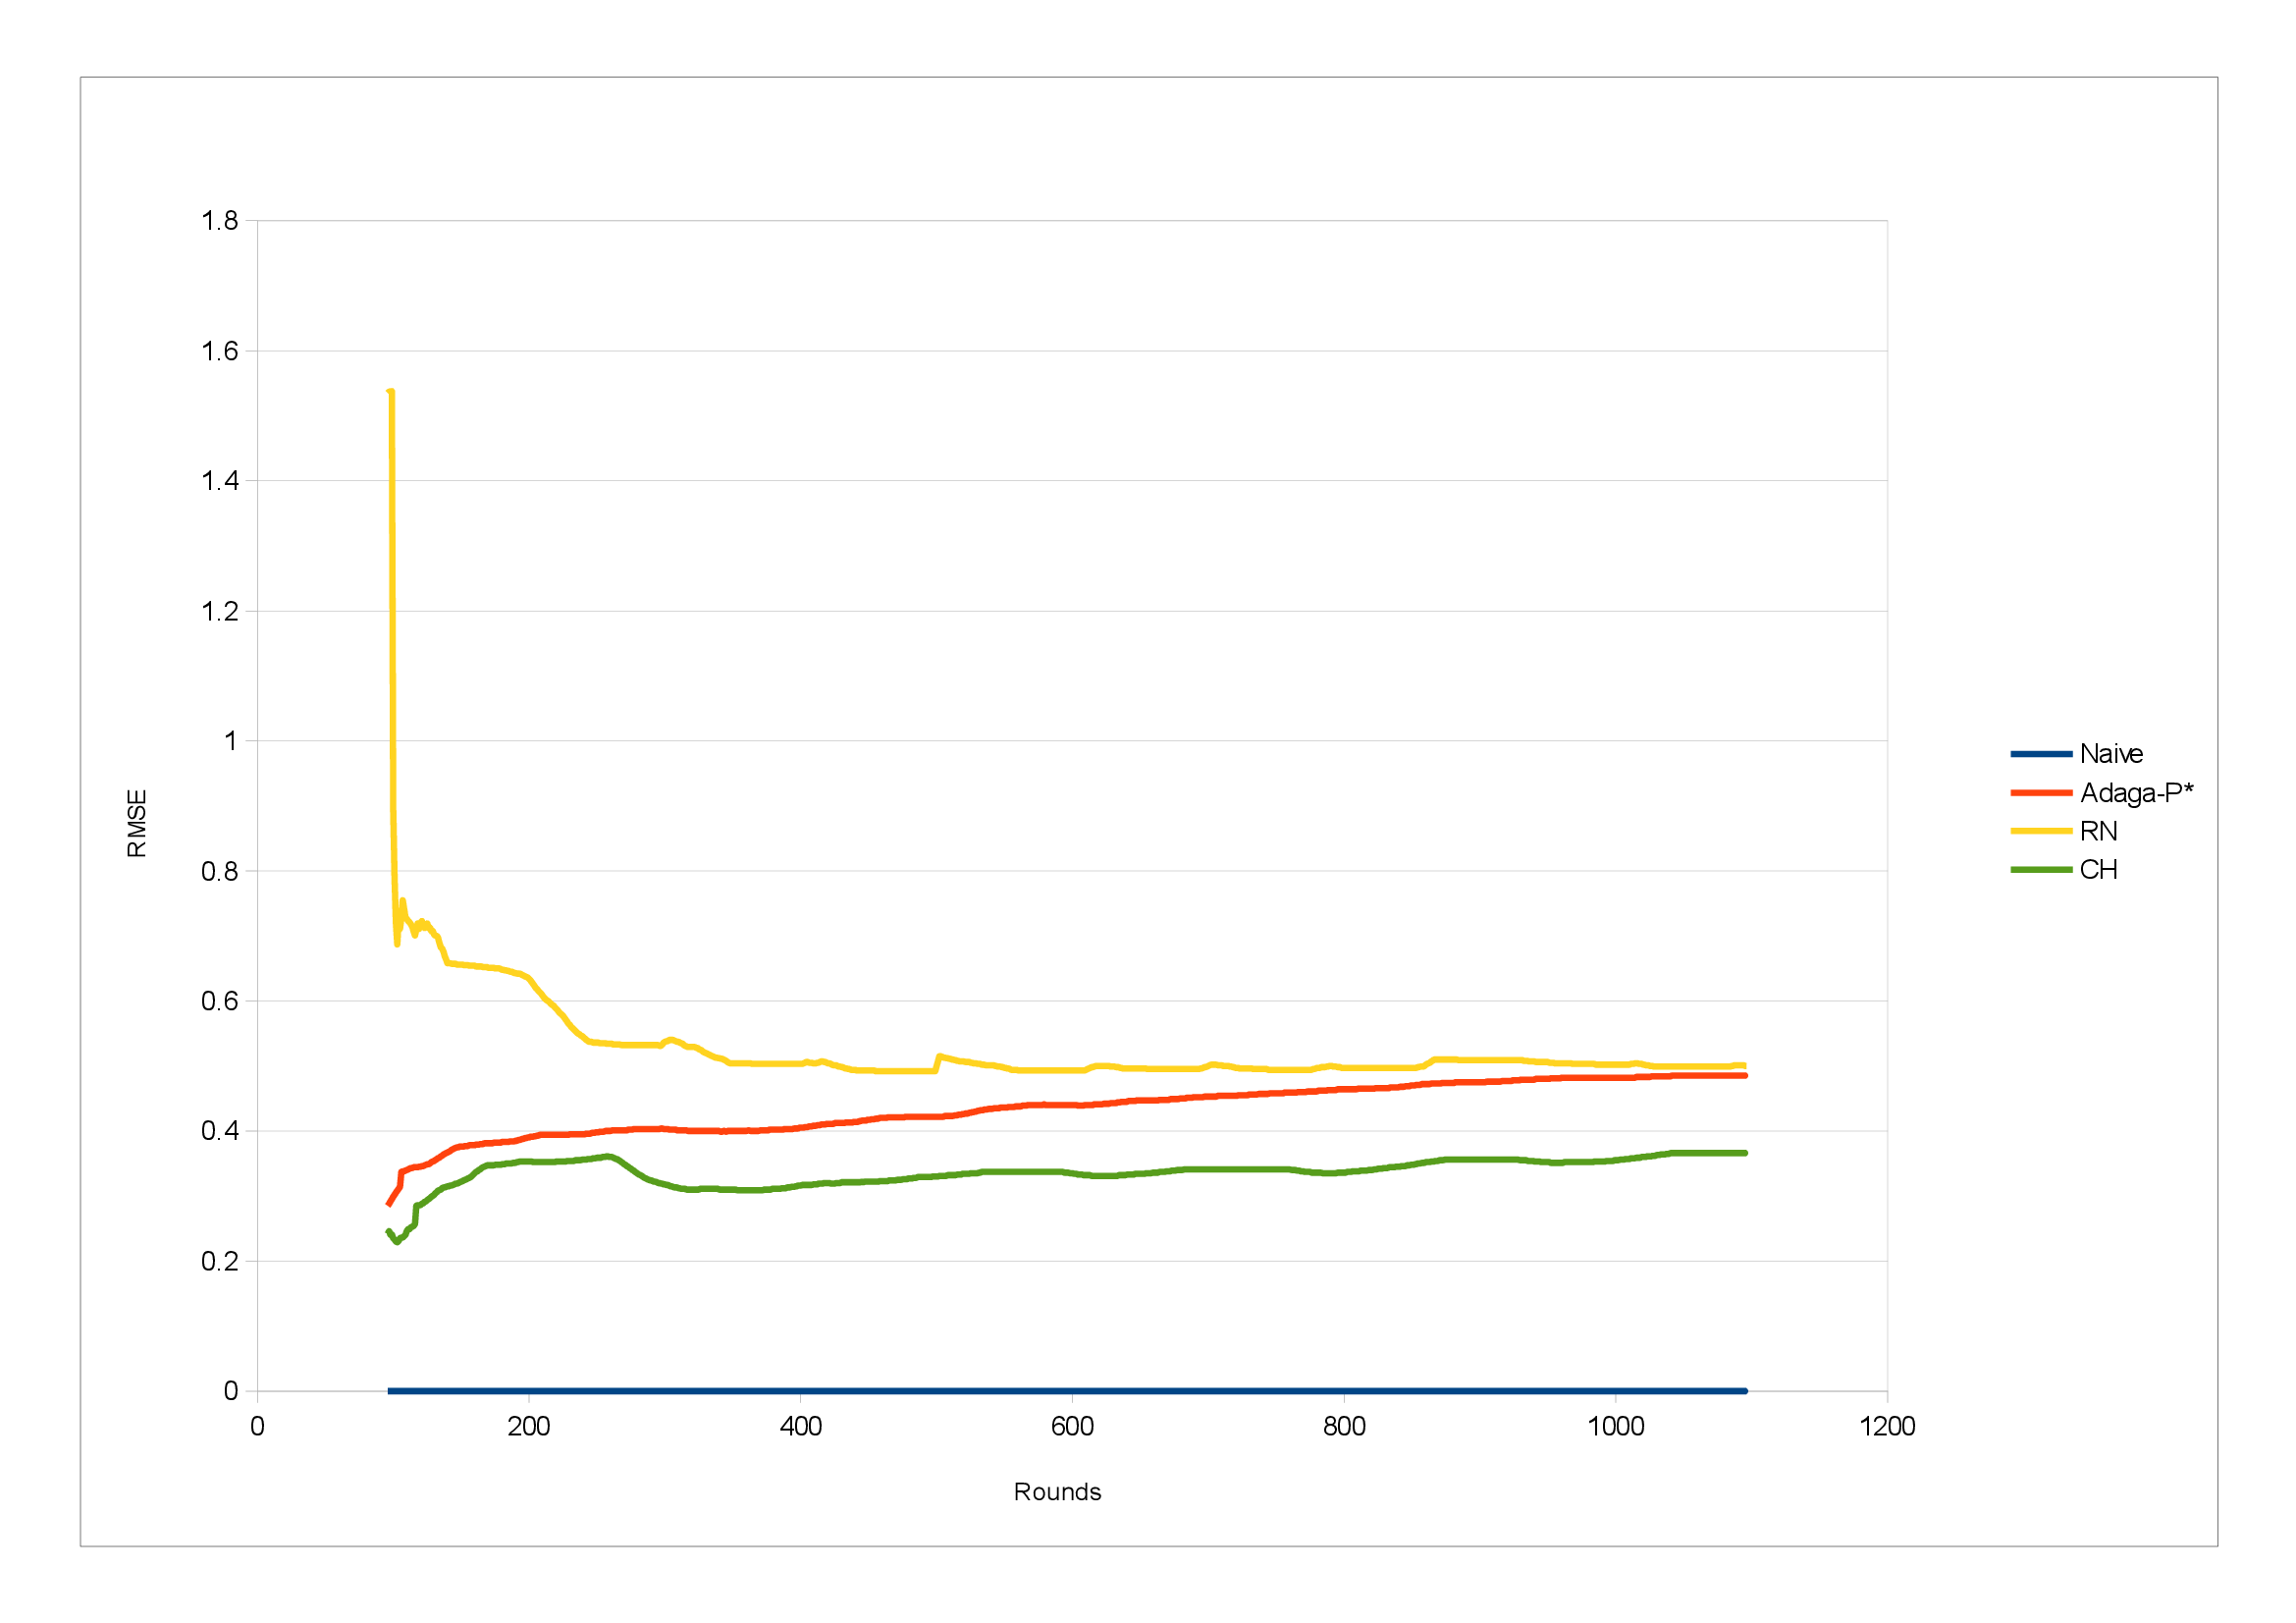
\includegraphics[scale=0.11]{RMSEGRAPHIC_.png}
    \caption{RMSE per Round}
    \label{fig:rmse}
\end{figure}

One can identify a peak in Figure \ref{fig:rmse} for the BCWSN-RN curve. The
reason for that is the following. After the initial cluster formation there is a
small number of clusters and in the BCWSN-RN just the representative nodes are
responsible for sensing data. Since there is only one representative node per
cluster, the number of sensed data is small as well. Thus the BCWSN-RN accuracy
is jeopardized at the beginning. Nonetheless, the BCWSN-RN approach is able to
dynamically adjust the accuracy by reducing the RMSE.

In Figure \ref{fig:num-msg}, one can observe the number of transmitted messages
per round.
In the Naive approach, the number of messages is steady, since in each round all
sensors send sensed data to the sink.
It is important to observe that, in average, BCWSN-CH and BCWSN-RN transmit less
messages than Adaga-P* (see Table \ref{tab:num-msg}). However, there are some
peaks in both curves (BCWSN-CH and BCWSN-RN), which represents periods in time
when clusters are being restructured (splitting or merging). This can be proved
by the high standard deviation for both approaches in Table \ref{tab:num-msg}.

\begin{figure}[!htb]
\begin{center}
	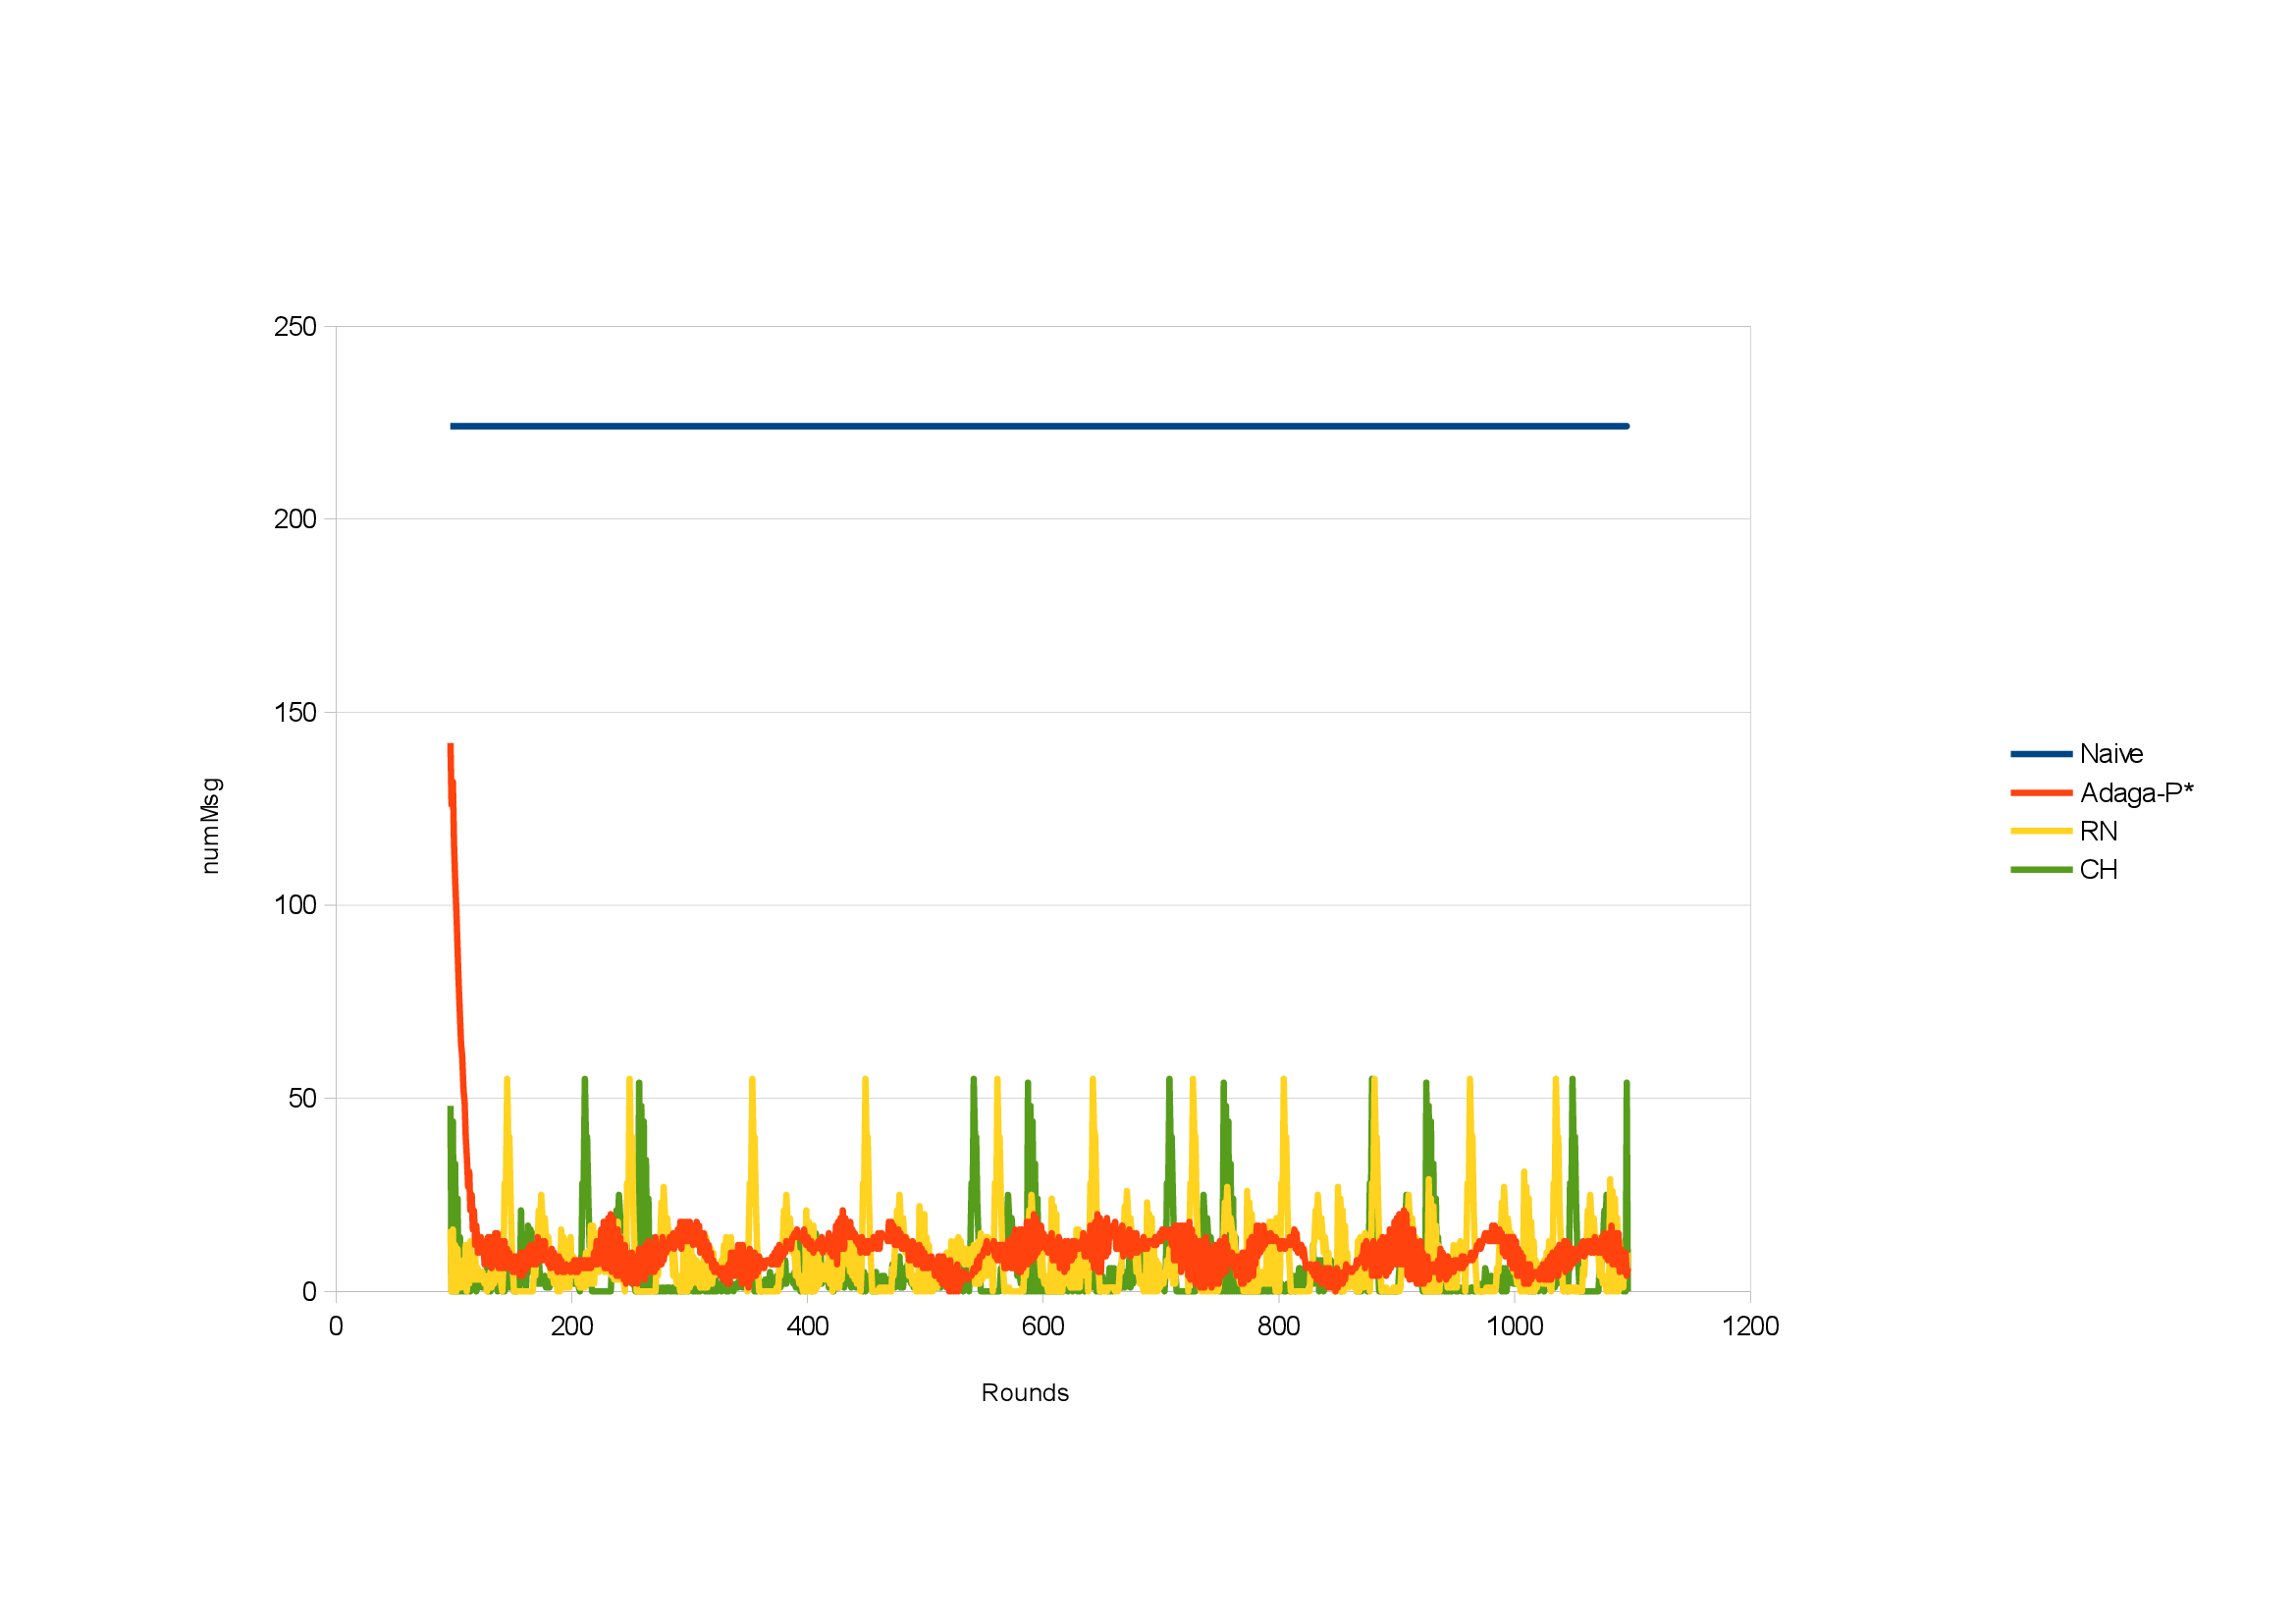
\includegraphics[scale=0.11]{NumMsgGRAPHIC_.png}
    \caption{Number of Messages per Round}
    \label{fig:num-msg}
\end{center}
\end{figure}


Finally, Figure \ref{fig:sens-reading} shows the evolution of the amount of
sensed data for the four evaluated approaches.
Naive and Adaga-P* approaches, as one can observe, have the same number of
sensed data (53 per round), because all sensors in those approaches sense data
during all cycles. In BCWSN-CH, sensors do not sense while they are waiting to
receive new coefficients after sending novelties to sink. In the case of
BCWSN-RN, only representative nodes (one per cluster) sense data per round.

\begin{figure}[!htb]
\centering
	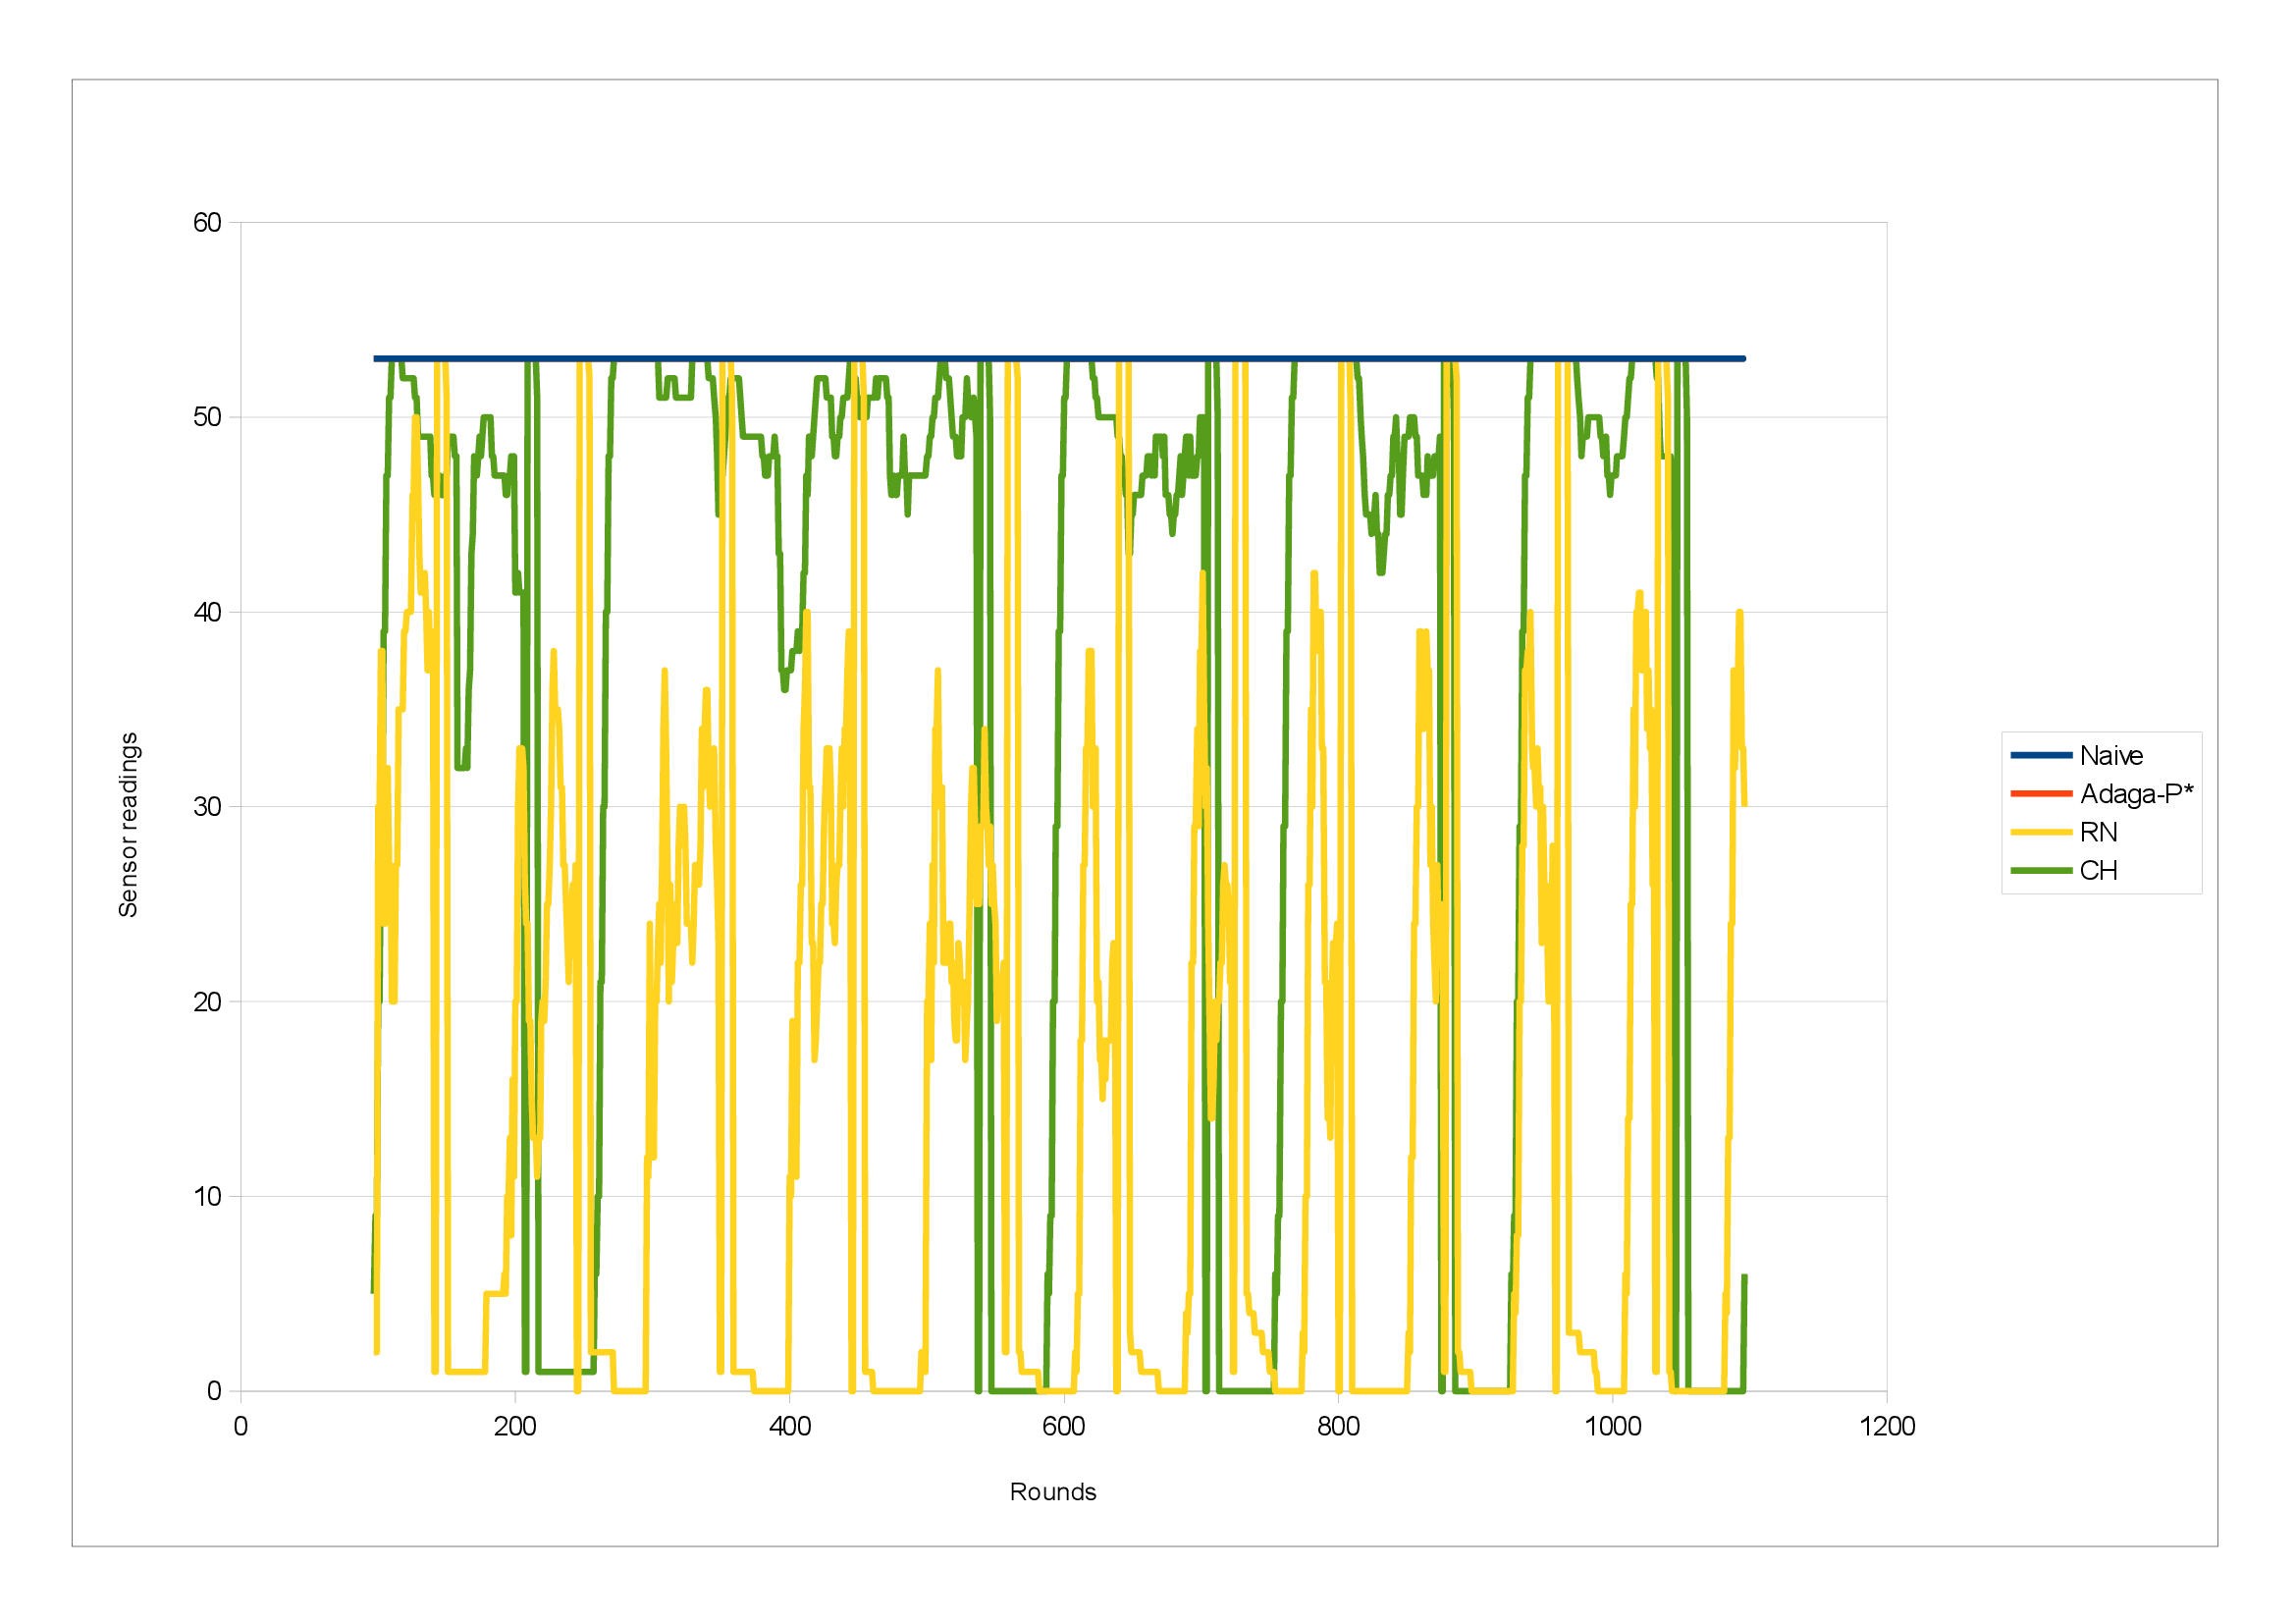
\includegraphics[scale=0.11]{SReadGRAPHIC_.png}
    \caption{Number of Sensed Data per Round}
    \label{fig:sens-reading}
\end{figure}


\section{Conclusion}
\label{conclusion}

In this paper, we have described a new approach for clustering sensors in WSNs
based on the notion of behavioral correlation. Behavioral correlation identifies
sensors with similar data reading patterns. Moreover, two different approaches
to select of active nodes in each cluster have been proposed:
Representative Nodes (RNs) and Cluster Heads (CHs).

The results presented in Section \ref{results-and-discussion} show that the use
of data behavioral correlation associated with a temporal correlation technique
may significantly increase energy economy in WSNs, while assuring a low RMS
Error.

In this work, the similarity among time series behavior has been measured by
applying similarity in magnitude and trend. Now, we are working on evaluating
measures of distance between prediction models to assess the dissimilarity in
sensed data behavior.


% conference papers do not normally have an appendix



\bibliographystyle{IEEEtran}
\bibliography{IEEEabrv,ISCC2014rodrigues_brayner_maia}  
% ISCC2014rodrigues_brayner_maia.bib is the name of the Bibliography in this case
% You must have a proper ".bib" file
%  and remember to run:
% latex bibtex latex latex
% to resolve all references

\end{document}


